

\begin{frame}{Game Theory} 

    \textbf{What is game theory?}

    It is the study of mathematical models of strategic interactions. 

    \begin{columns}
        \begin{column}{0.5\textwidth}

            \begin{figure}
                \centering
                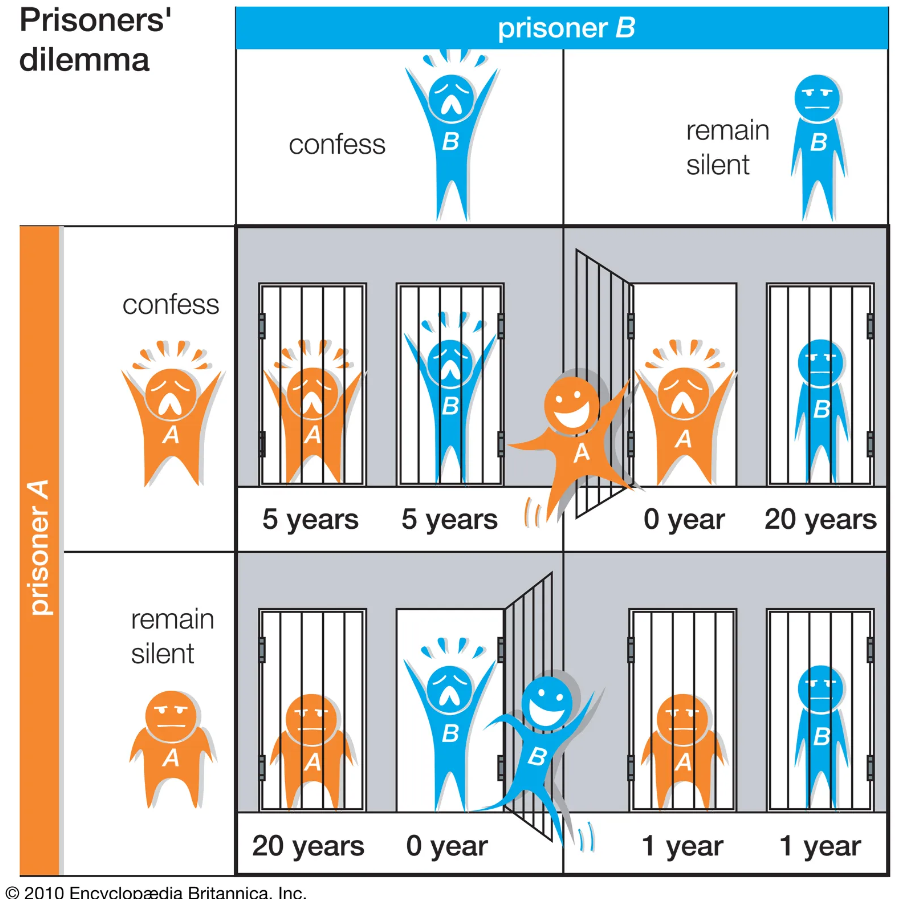
\includegraphics[width=\textwidth]{pres_images/prisoners_dilemma.png}
                \caption{Prisoner's Dilemma}
                \label{fig:enter-label}
            \end{figure}                
            
        \end{column}
        \begin{column}{0.4\textwidth}

            \begin{align*}
            A & = \begin{bmatrix} 
                    5 & 0 \\ 
                    20 & 1 
                \end{bmatrix} \\ 
                B = A^\top & = \begin{bmatrix}
                    5 & 20 \\ 
                    0 & 1 
                \end{bmatrix}
            \end{align*}
            
        \end{column}
    \end{columns}

\end{frame}

\begin{frame}{Game Theory}

    The \textbf{maximin} value is 
    \begin{itemize}
        \item the highest value that the player can be given worst-case actions by other players  
    \end{itemize} 
    
    \begin{equation}
        \underline{v_i} = \max_{a} \min_{a_{-i}} v_i ( a_i, a_{-i} )
    \end{equation}

    where 
    \begin{itemize}
        \item $i$ is the player 
        \item $-i$ denotes all players except $i$ 
        \item $a_i$ is action taken by player $i$ 
        \item $a_{-i}$ denotes actions taken by other players 
        \item $v_i$ is value function for player $i$ 
    \end{itemize}
    
\end{frame} 

\begin{frame}{Game Theory} 

    The \textbf{Nash equilibrium} is a situation where no player could gain by changing their own strategy (all other players' strategies fixed). 

    In two-player zero-sum games, the maximin solution is the same as the Nash equilibrium.

    John F. Nash, Jr. won the Nobel prize for proving: 
    \begin{itemize}
        \item for games with finite players and pure strategies 
        \item if \textbf{mixed strategies} are allowed 
        \item every game has \textbf{at least one equilibrium} 
    \end{itemize}
    
\end{frame} 

\begin{frame}{Pursuit Evasion Game} 

    To lift the pursuit evasion game from the planar environment to a 3-dimensional game subject to orbital dynamics constraints, a local reference frame for a 6-sided polygon was first defined. The polygon is centered along the reference trajectory. 

    \begin{figure}
        \centering
        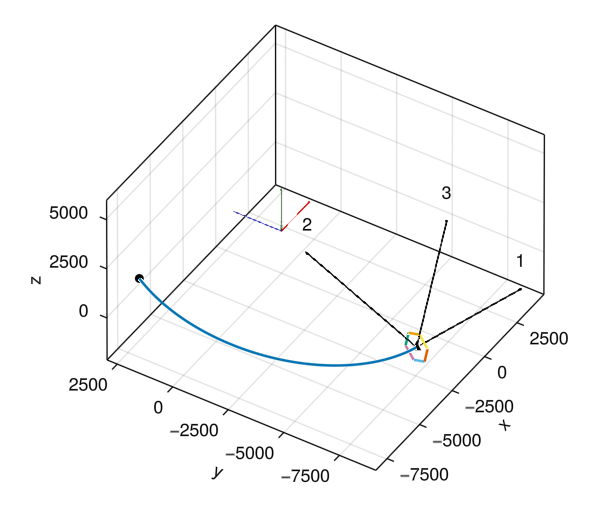
\includegraphics[width=0.5\textwidth]{pres_images/polygon_define.png}
        \caption{Polygon definition}
        \label{fig:polygon_definition}
    \end{figure}
    
\end{frame} 

\begin{frame}{Pursuit Evasion Game} 

    Then, trajectories targeting the 6 vertices of the polygon were computed. 

    \begin{figure}
    \centering
    \begin{minipage}{0.6\textwidth}
        \centering
        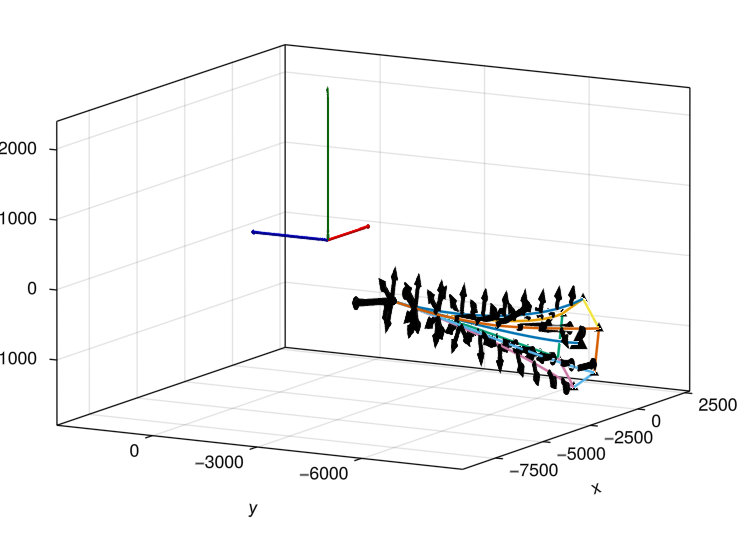
\includegraphics[width=\linewidth]{pres_images/polygon_6trajs.png}
        \caption{6 Trajectories}
    \end{minipage}\hfill
    \begin{minipage}{0.3\textwidth}
        \centering
        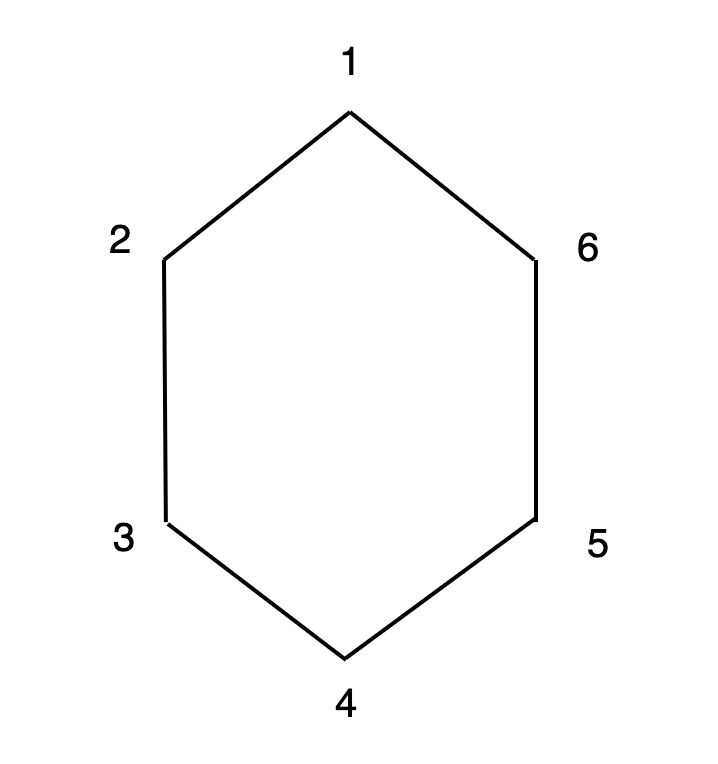
\includegraphics[width=\linewidth]{pres_images/hexagon_vertices.png}
        \caption{Vertex Labels}
    \end{minipage}
\end{figure}

    % \begin{figure}
    %     \centering
    %     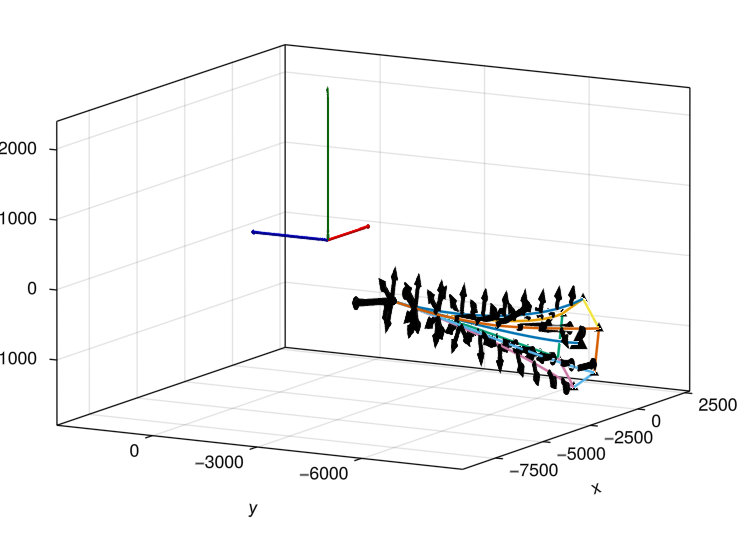
\includegraphics[width=0.5\textwidth]{pres_images/polygon_6trajs.png}
    %     \caption{Spacecraft targeting 6 vertices of polygon}
    %     \label{fig:polygon_targeting}
    % \end{figure}

    % \begin{figure}
    %     \centering
    %     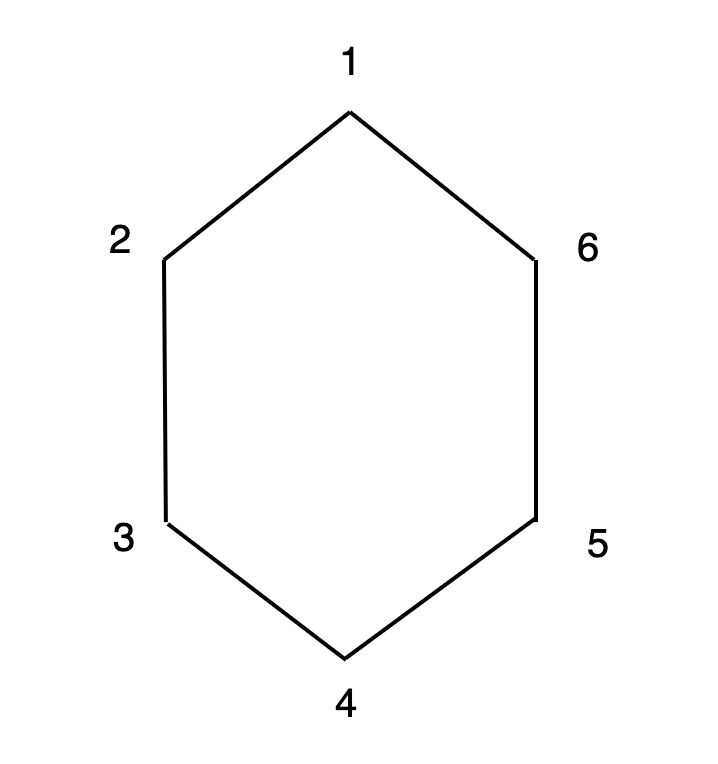
\includegraphics[width=0.5\linewidth]{pres_images/hexagon_vertices.png}
    %     \caption{Caption}
    %     \label{fig:placeholder}
    % \end{figure}
    
\end{frame}

\begin{frame}{Pursuit Evasion Game} 

    Trajectories targeting the 6 vertices of the polygon were computed for a pursuer and evader. 

    \begin{figure}
        \centering
        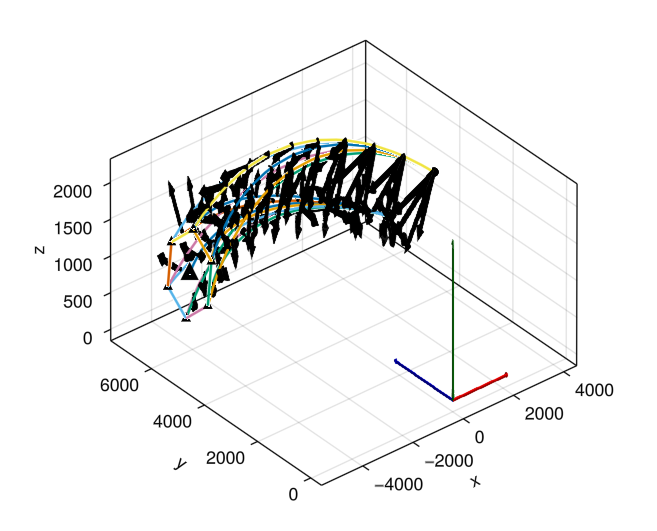
\includegraphics[width=0.5\textwidth]{pres_images/polygon_2agents.png}
        \caption{Spacecraft pursuer and evader targeting 6 vertices of polygon}
        \label{fig:polygon_targeting_pursuit_evasion}
    \end{figure}
    
\end{frame} 

\begin{frame}{Pursuit Evasion Game} 

    The stage cost at each time instant was computed and then averaged along the entire trajectory. 
% 
    \begin{equation}
        \text{cost}(t) = \sqrt{ || \mathbf{r}_1(t) - \mathbf{r}_2(t) ||_2 + 0.1 } + 0.1 ( || \mathbf{u}_1(t) ||_2 - || \mathbf{u}_2(t) ||_2 )
    \end{equation} 
% 
    The average stage cost $C_{ij}$ was then saved in a cost matrix for each $i,j $ trajectory / vertex pairing. This results in a 6x6 cost matrix:  
% 
    \begin{equation}
        A = 
        \begin{bmatrix}
            C_{11} & C_{12} & \ldots & C_{16} \\ 
            \vdots & \vdots &        & \vdots \\ 
            C_{61} & C_{62} & \ldots & C_{66} 
        \end{bmatrix}
    \end{equation}

    We are playing a zero sum game, so the cost matrix for one player is equivalent to the negative of the cost matrix for the other player. 
    
\end{frame} 

\begin{frame}{Pursuit Evasion Game} 

    % To solve the mixed strategy problem and find weights for each trajectory, we first transform the game to ensure that the cost matrix is entrywise positive. 
    We then transform the game to ensure that the cost matrix is entrywise positive and solve the linear program associated with a zero sum game 
    % 
    \begin{align}
        \max_{ \mathbf{z} \in \mathbb{R}^6 }    & \; \; \mathbf{1}^T \mathbf{z} \\ 
        \text{ subject to }                     & \; \; \mathbf{1} \geq A^T \mathbf{z}    
    \end{align} 

    Finally, we turn the solution into a probability simplex, resulting in mixing weights $ x^* $ for each trajectory / vertex for each player 

    \begin{equation}
        x^*         & = \frac{\mathbf{z^*}}{ \mathbf{1}^T \mathbf{z^*} }  
    \end{equation} 

    To play the game, we sample from the mixing weights for each player. 
    
\end{frame} 




